\newpage
\changeindent{0cm}
\section{数値実験}
\label{sec:exp}
\changeindent{2cm}


\changeindent{0cm}
\subsection{提案手法:DARTS}
\label{sec:exp.01}
\changeindent{2cm}

\begin{table}[b]
  \begin{center}
    \caption{実験1 : 各アーキテクチャの精度}
		\vspace{3mm}
    \begin{tabular}{|c|c|c|c|c|c|}\hline
    \multicolumn{2}{|c|}{\textbf{architecture}} & \textbf{\begin{tabular}[c]{@{}c@{}}test accuracy\\ (\%)\end{tabular}} & \textbf{\begin{tabular}[c]{@{}c@{}}param\\ (M)\end{tabular}} & \textbf{\begin{tabular}[c]{@{}c@{}}shortcut # \end{tabular}} & \textbf{\begin{tabular}[c]{@{}c@{}}random architect\\ accuracy (\%)\end{tabular}} \\ \hline
    \multirow{3}{*}{\begin{tabular}[c]{@{}c@{}}method A\end{tabular}} & 50 epoch & 93.70 $\pm$ 0.22 & 21.06 $\pm$ 0.07 & 12.7 $\pm$ 1.4 & 93.60 $\pm$ 0.15 \\ \cline{2-6}
     & 100 epoch & 94.02 $\pm$ 0.12 & 21.50 $\pm$ 0.11 & 18.2 $\pm$ 0.9 & 93.67 $\pm$ 0.14 \\ \cline{2-6}
     & 150 epoch & 93.90 $\pm$ 0.17 & 21.57 $\pm$ 0.25 & 18.9 $\pm$ 0.6 & 93.64 $\pm$ 0.09 \\ \hline
    \multirow{3}{*}{\begin{tabular}[c]{@{}c@{}}method B\end{tabular}} & 50 epoch & 93.57 $\pm$ 0.19 & 20.45 $\pm$ 0.09 & 5.8 $\pm$ 1.2 & 93.36 $\pm$ 0.19 \\ \cline{2-6}
     & 100 epoch & 93.93 $\pm$ 0.08 & 20.73 $\pm$ 0.10 & 9.8 $\pm$ 1.0 & 93.47 $\pm$ 0.17 \\ \cline{2-6}
     & 150 epoch & 93.92 $\pm$ 0.12 & 20.76 $\pm$ 0.15 & 10.6 $\pm$ 1.0 & 93.48 $\pm$ 0.15 \\ \hline
    \multicolumn{2}{|c|}{baseline (VGG19)} & 93.03 $\pm$ 0.10 & 20.04 & 0 & - \\ \hline
    \end{tabular}
    \label{tab:accg}
  \end{center}
\end{table}

表 \ref{tab:accg} に各構成手法におけるテストデータの精度を示す.
図 \ref{fig:short}, \ref{fig:param} には
表 \ref{tab:accg} の精度に対するショートカット数とパラメータ数の関係を図示する.
最も性能が高かったのは100 epoch 時点の手法Aで94.02 \%(baseline+0.99\%)となり,
100 epoch 時点の手法Bは93.93 \%(baseline+0.90\%)となった.
しかしランダム手法と比較すると, 手法Aは+0.35\%, 手法Bは+0.46\%となり,
図 \ref{fig:param} を参照しても少ないパラメータ数でより有効に探索できているのは手法Bと言える.

また100 epoch時点と150 epoch時点を比較すると, 学習によって性能が悪化している.
問題に対して過度に適合していることが原因であると考えられる.

探索時間は150 epochでおよそ 5 GPU hours を要したが, DARTSと比べ演算子を探索していないことや.
最適な重み $w^*$ の近似を1次下げていることで高速になったと思われる.

図 \ref{fig:exp1_a}, \ref{fig:exp1_b} には, 手法A, Bのアーキテクチャの 50 epoch ごとの
結果として, 10回試行のうちの1つを示した.
ランダム探索では見られなかったような, 比較的離れた位置からの接続が多いという特徴があった.
さらに, 学習を経るごとに離れていくため, 接続の距離がネットワークの性能に関係していると考えられる.
これは離れた位置からの接続が, あまり変換されていない特徴の情報を引き継げることが,
性能向上の要因と解釈できる.


% ここで 0.5 Page



\begin{figure}[t]
  \begin{center}
    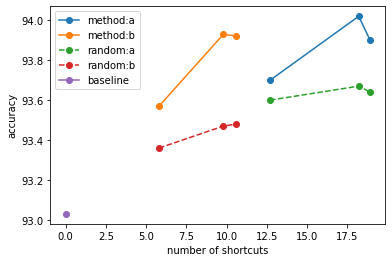
\includegraphics[clip,width=10cm]{./fig/short.png}
  \end{center}
  \caption{実験1 : ショートカット数に対する精度}
  \label{fig:short}
\end{figure}
\begin{figure}[t]
  \begin{center}
    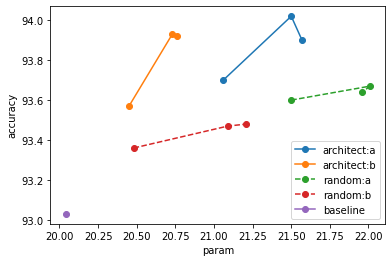
\includegraphics[clip,width=10cm]{./fig/param.png}
  \end{center}
  \caption{実験1 : パラメータ数に対する精度}
  \label{fig:param}
\end{figure}


\begin{figure}[tb]
 \begin{minipage}{0.3\hsize}
 	\begin{center}
 		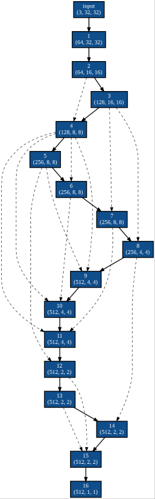
\includegraphics[clip,scale=0.8]{./fig/04.exp/a50.png}\\
 		50 epoch
 	\end{center}
 \end{minipage}
 \begin{minipage}{0.3\hsize}
 	\begin{center}
    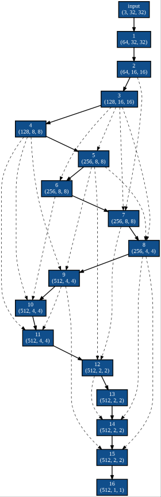
\includegraphics[clip,scale=0.8]{./fig/04.exp/a100.png}\\
    100 epoch
 	\end{center}
 \end{minipage}
 \begin{minipage}{0.3\hsize}
 	\begin{center}
    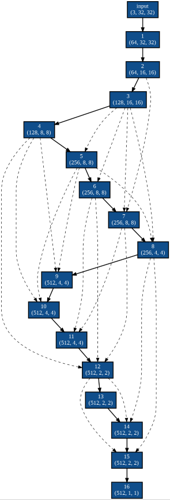
\includegraphics[clip,scale=0.8]{./fig/04.exp/a150.png}\\
    150 epoch
 	\end{center}
 \end{minipage}
 \caption{実験1 : 手法Aのアーキテクチャ 例}
 \label{fig:exp1_a}
\end{figure}


\begin{figure}[tb]
 \begin{minipage}{0.3\hsize}
 	\begin{center}
 		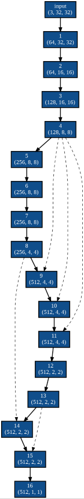
\includegraphics[clip,scale=0.8]{./fig/04.exp/b50.png}\\
 		50 epoch
 	\end{center}
 \end{minipage}
 \begin{minipage}{0.3\hsize}
 	\begin{center}
    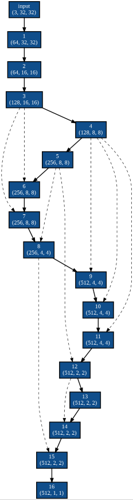
\includegraphics[clip,scale=0.8]{./fig/04.exp/b100.png}\\
    100 epoch
 	\end{center}
 \end{minipage}
 \begin{minipage}{0.3\hsize}
 	\begin{center}
    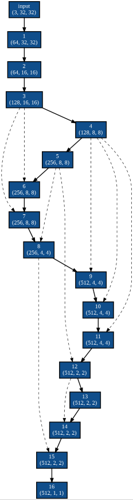
\includegraphics[clip,scale=0.8]{./fig/04.exp/b150.png}\\
    150 epoch
 	\end{center}
 \end{minipage}
 \caption{実験1 : 手法Bのアーキテクチャ 例}
 \label{fig:exp1_b}
\end{figure}





\clearpage\newpage
\changeindent{0cm}
\subsection{提案手法:DARTS+TDGA}
\label{sec:exp.02}
\changeindent{2cm}

3つの提案手法の最終的なアーキテクチャ性能はこの表のようになりました.
50世代ごとの結果全てに対して, DARTSのみとなる事前学習のアーキテクチャ 93.65\%をいずれも超えることができました.
この表を横軸が世代数 縦軸がaccuracyの図にすると, wを更新する青色の提案手法1が150世代目で性能が下がっています. またDARTSの更新をしない緑色の提案手法3が最もよい結果となりました.

この結果からDARTSによる頻繁な更新がTDGAの正確な適応度計算を妨害していることが原因として考えられます
.

表 \ref{tab:acc_ga}.
図 \ref{fig:exp2/eval},
図 \ref{fig:exp2/acc},
図 \ref{fig:exp2/loss},
図 \ref{fig:exp2/edge},

図 \ref{fig:exp2/archi}, \ref{fig:exp2/archi2}.

% ここで 1 Page


\begin{table}[t]
  \begin{center}
    \caption{実験2 : 各提案手法のアーキテクチャ性能}
		\vspace{-1mm}
    ベースラインは事前学習時のネットワーク.
		\vspace{1mm}
		\vspace{3mm}
    \begin{tabular}{|c|c|c|c|} \hline
    \textbf{}       & \textbf{50 世代} & \textbf{100 世代} & \textbf{150 世代} \\ \hline\hline
    DAARTS + TDGA($w$, $\alpha$)& 94.03 \%       & 94.10 \%        & 93.85 \%        \\ \hline
    DAARTS + TDGA($\alpha$)& 93.88 \%       & 94.08 \%        & 94.13 \%        \\ \hline
    DAARTS + TDGA   & 93.90 \%       & 94.17 \%        & 94.17 \%        \\ \hline
    Baseline(DARTS) & \multicolumn{3}{c|}{93.65 \%}                      \\ \hline
    \end{tabular}
    \label{tab:acc_ga}
  \end{center}
\end{table}

\begin{figure}[t]
  \begin{center}
    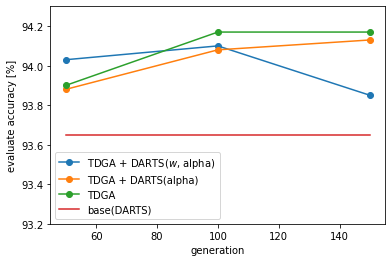
\includegraphics[clip,width=10cm]{./fig/04.exp/eval.png}
  \end{center}
  \caption{実験2 : 各提案手法のアーキテクチャ性能}
  \label{fig:exp2/eval}
\end{figure}
\begin{figure}[t]
  \begin{center}
    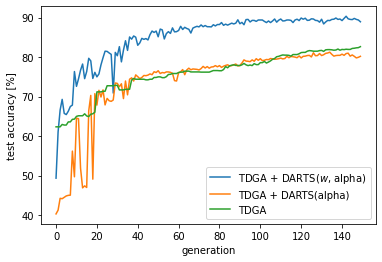
\includegraphics[clip,width=10cm]{./fig/04.exp/acc.png}
  \end{center}
  \caption{実験2 : 各提案手法の探索時の正解率}
  \label{fig:exp2/acc}
\end{figure}
\begin{figure}[t]
  \begin{center}
    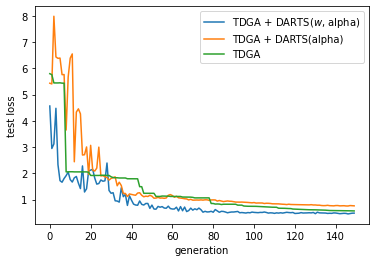
\includegraphics[clip,width=10cm]{./fig/04.exp/loss.png}
  \end{center}
  \caption{実験2 : 各提案手法の探索時の損失}
  \label{fig:exp2/loss}
\end{figure}
\begin{figure}[t]
  \begin{center}
    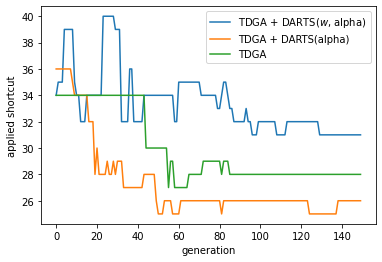
\includegraphics[clip,width=10cm]{./fig/04.exp/edge.png}
  \end{center}
  \caption{実験2 : 各提案手法の探索過程のショートカット数}
  \label{fig:exp2/edge}
\end{figure}


\begin{figure}[tb]
 \begin{minipage}{0.5\hsize}
 	\begin{center}
    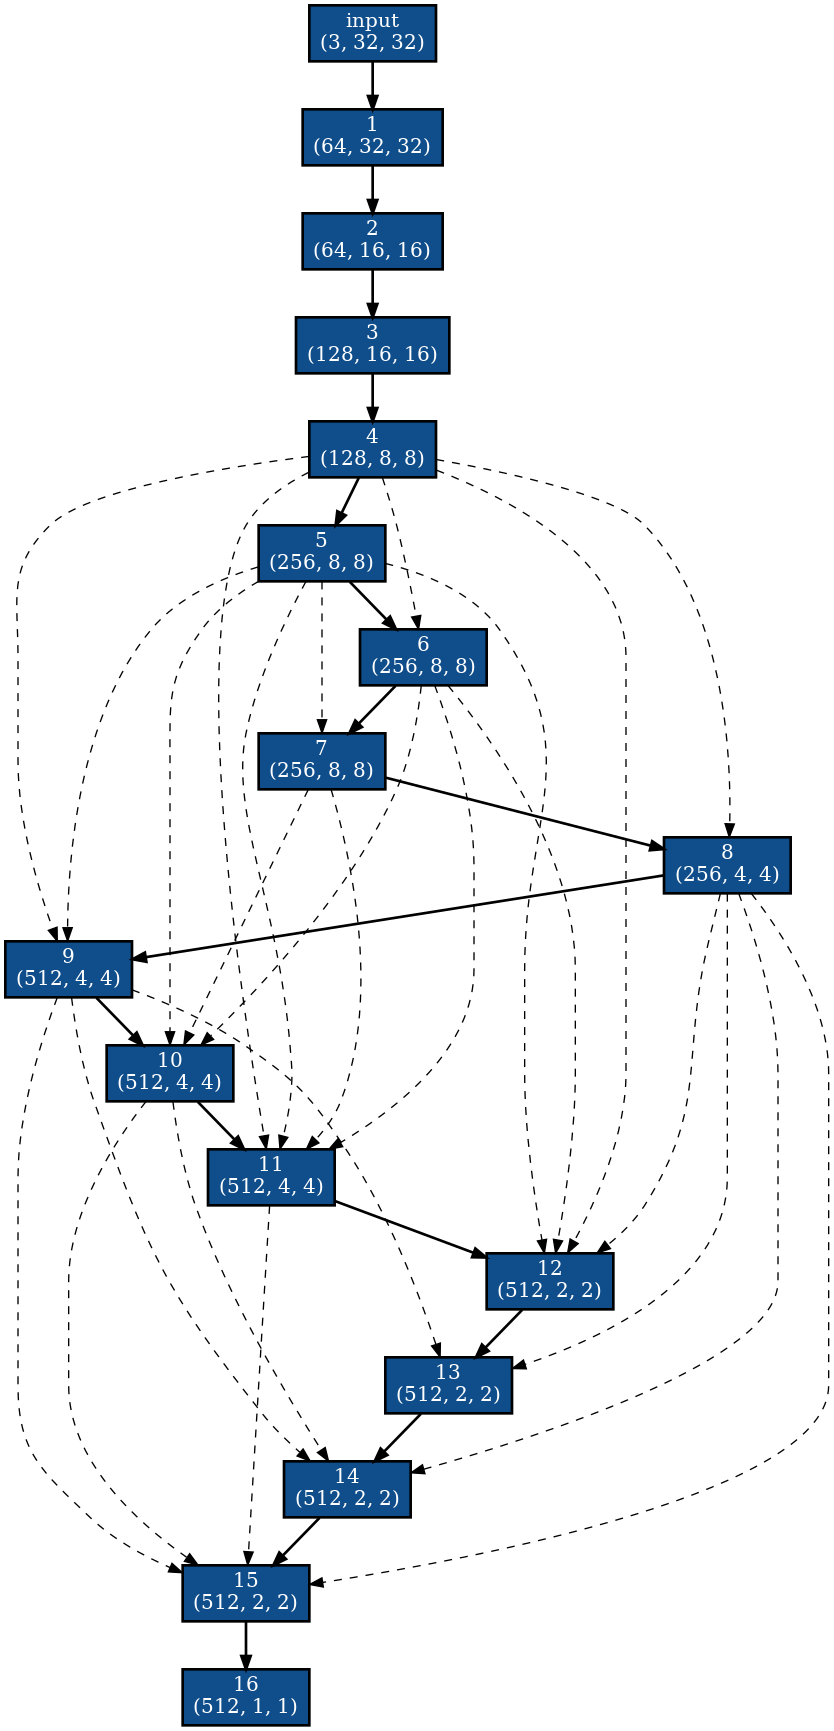
\includegraphics[clip,scale=0.2]{./fig/04.exp/base.png}\\
    Baseline (DARTS)
 	\end{center}
 \end{minipage}
 \begin{minipage}{0.5\hsize}
 	\begin{center}
    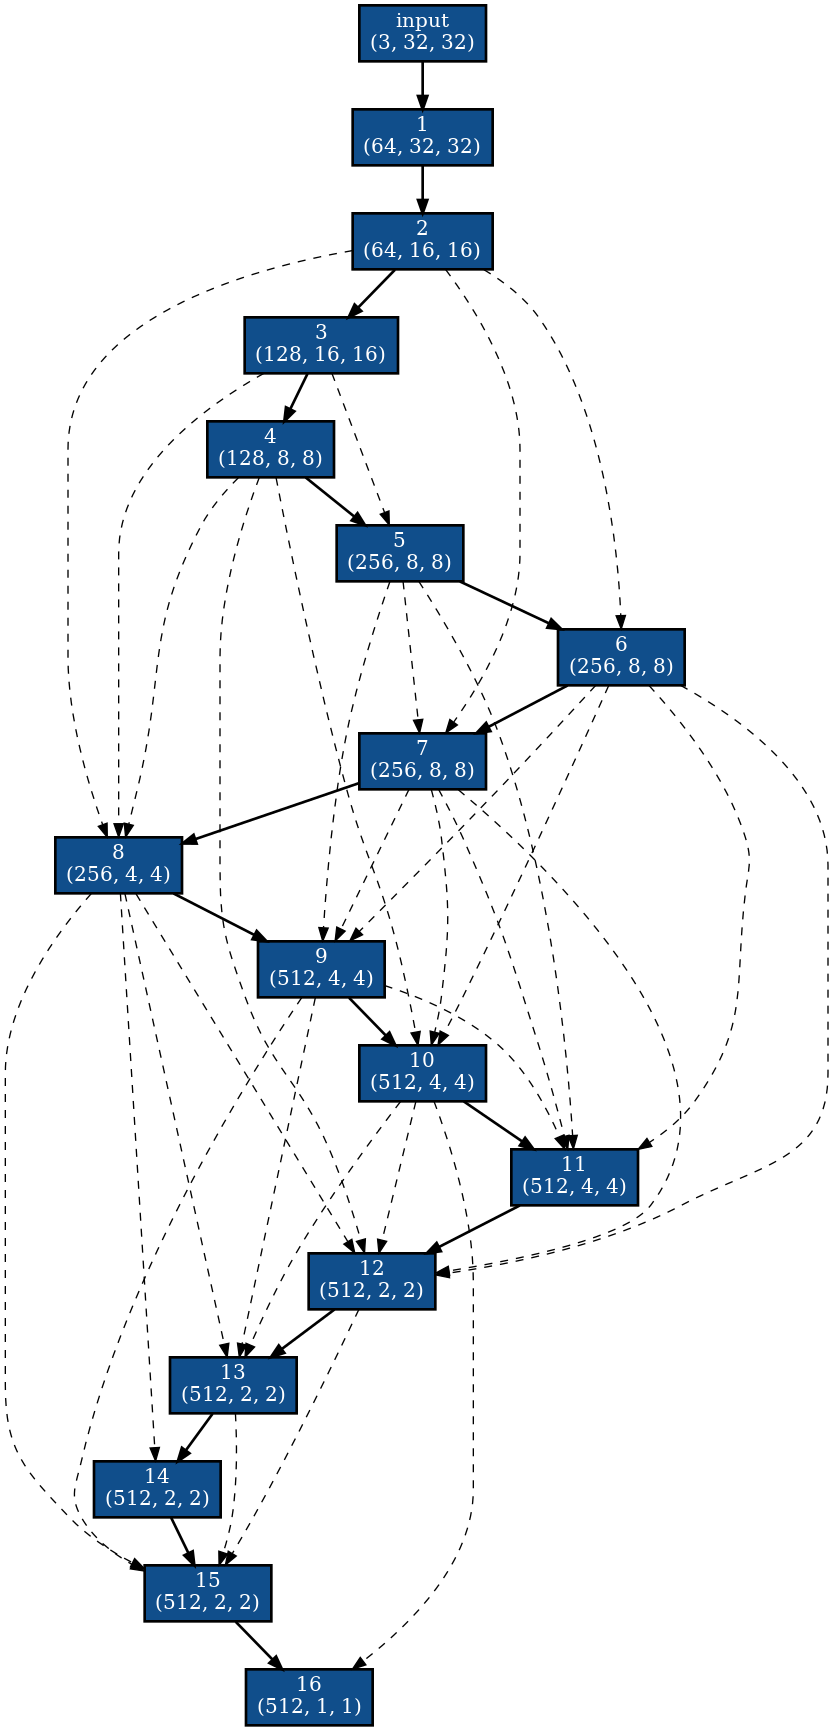
\includegraphics[clip,scale=0.2]{./fig/04.exp/nofix_last.png}\\
    DAARTS + TDGA($w$, $\alpha$)
 	\end{center}
 \end{minipage}
 \caption{実験2 : 手法のアーキテクチャ 1/2}
 \label{fig:exp2/archi}
\end{figure}

\begin{figure}[tb]
 \begin{minipage}{0.5\hsize}
 	\begin{center}
    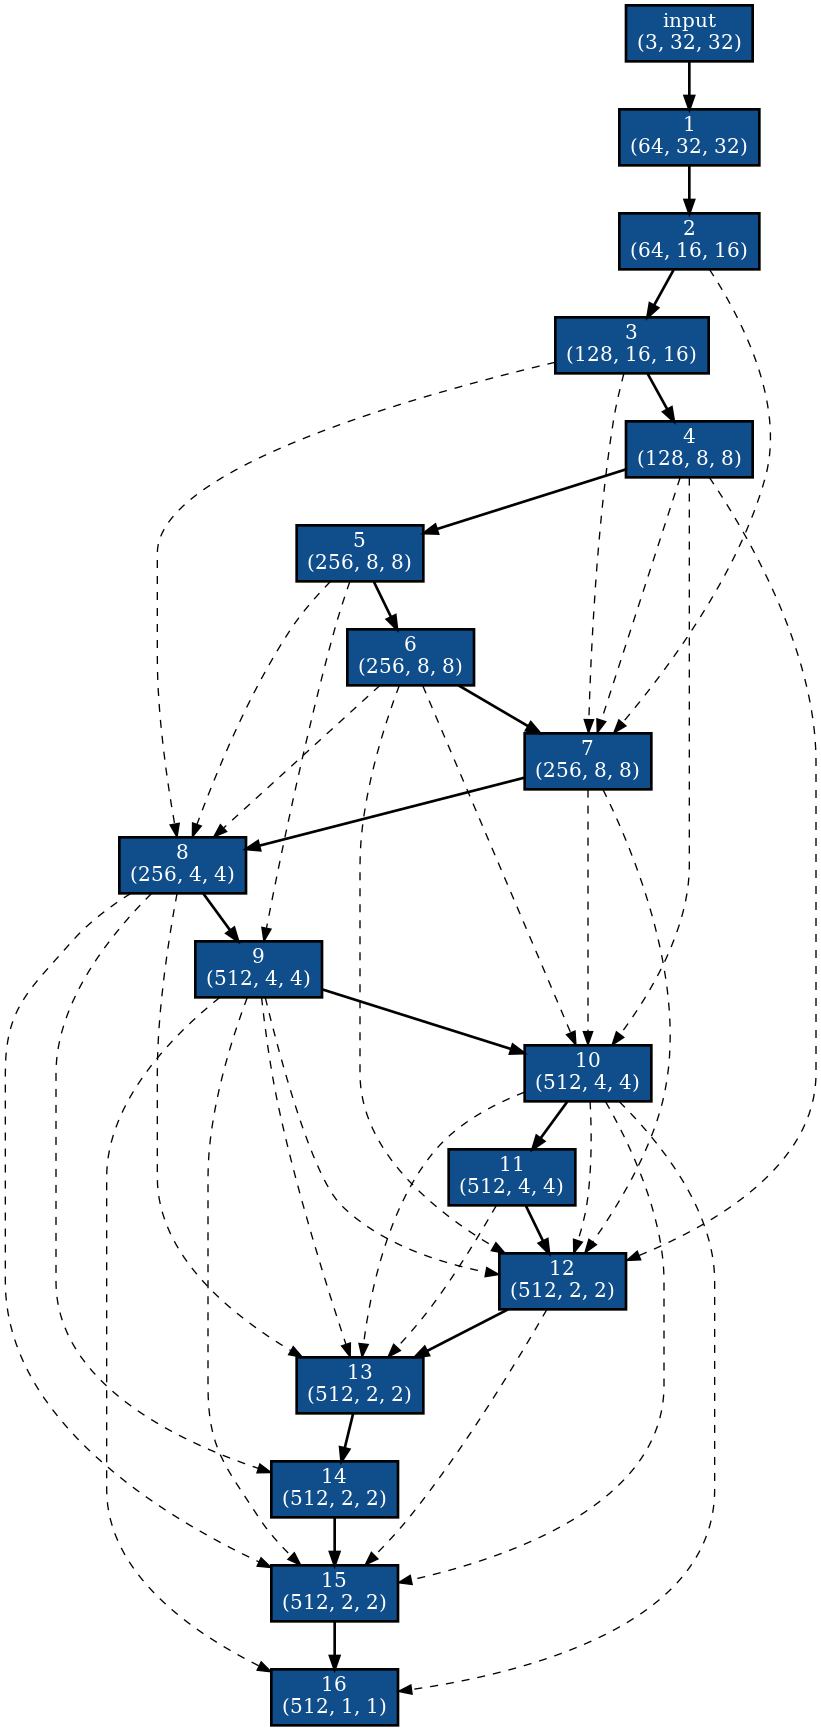
\includegraphics[clip,scale=0.2]{./fig/04.exp/normal_last.png}\\
    DAARTS + TDGA($\alpha$)
 	\end{center}
 \end{minipage}
 \begin{minipage}{0.5\hsize}
 	\begin{center}
    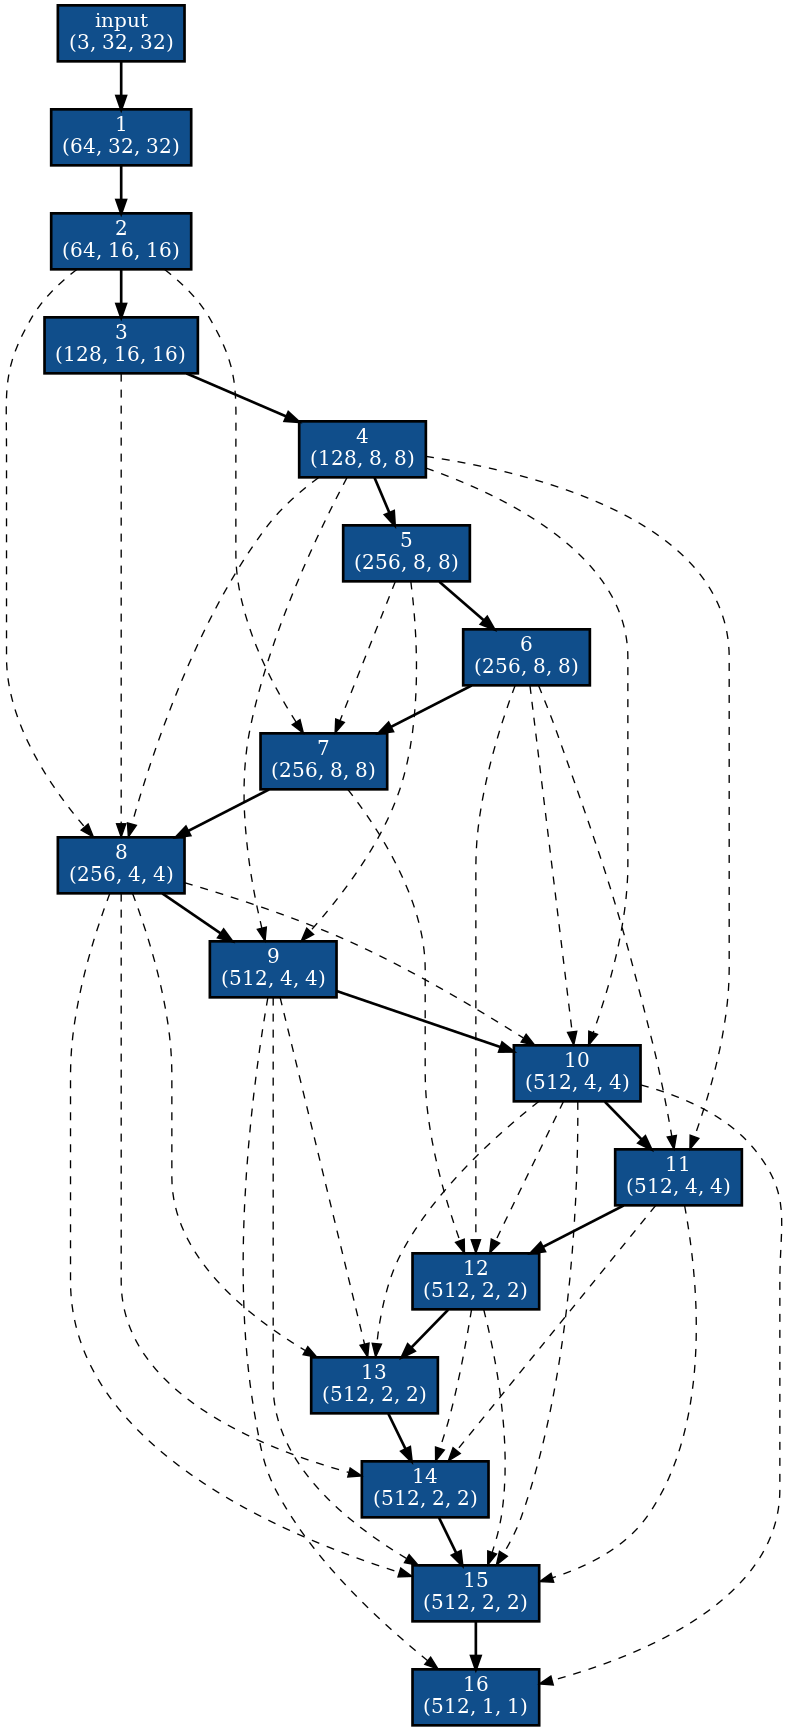
\includegraphics[clip,scale=0.2]{./fig/04.exp/noevo_last.png}\\
    DAARTS + TDGA
 	\end{center}
 \end{minipage}
 \caption{実験2 : 手法のアーキテクチャ 2/2}
 \label{fig:exp2/archi2}
\end{figure}

% \begin{figure}[t]
%   \begin{tabular}{cc}
%     \begin{minipage}[t]{0.5\hsize}
%     	\begin{center}
%         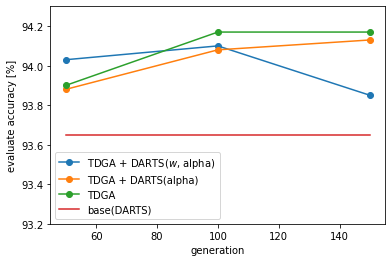
\includegraphics[clip, width=70mm]{./fig/04.exp/eval.png}\\
%         eval
%       \end{center}
%     \end{minipage}
%     \begin{minipage}[t]{0.5\hsize}
%     	\begin{center}
%         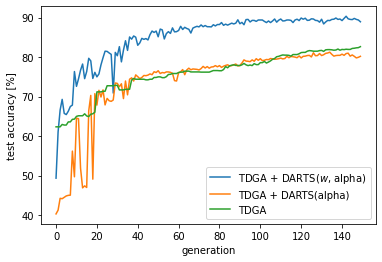
\includegraphics[clip, width=70mm]{./fig/04.exp/acc.png}\\
%         accuracy
%       \end{center}
%     \end{minipage}
%     \\
%     \begin{minipage}[c]{0.5\hsize}
%     	\begin{center}
%         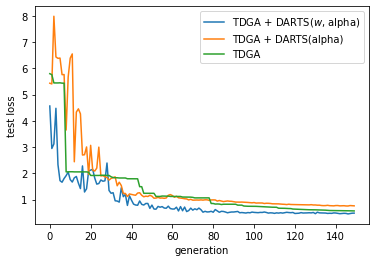
\includegraphics[clip, width=70mm]{./fig/04.exp/loss.png}\\
%         loss
%       \end{center}
%     \end{minipage}
%     \begin{minipage}[c]{0.5\hsize}
%     	\begin{center}
%         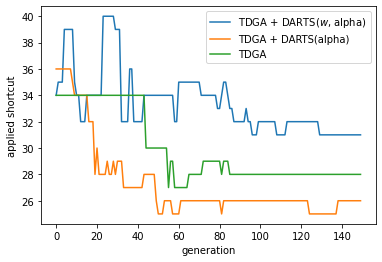
\includegraphics[clip, width=70mm]{./fig/04.exp/edge.png}\\
%         edge
%       \end{center}
%     \end{minipage}
%   \end{tabular}
%   \caption{実験2 : result}
%   \label{fig:exp2_graph}
% \end{figure}
